\subsection{Ottavo sprint}

\begin{minipage}{\textwidth}
  Di seguito è riportata la distribuzione delle ore per ciascun membro del team, accumulate in totali per persona e per ruolo:
  \begin{table}[H]
    \begin{tabularx}{\textwidth}{|c|*{6}{>{\centering}X|}c|}
      \hline
      \multicolumn{8}{|c|}{\textbf{Consuntivo orario}} \\
      \hline
      \textbf{Membro del team} & \textbf{Re} & \textbf{Am} & \textbf{An} & \textbf{Pt} & \textbf{Pr} & \textbf{Ve} & \textbf{Totale per persona} \\
      \hline
      Cavalli Riccardo & 0 & 0 & 0 & 0 & 2 & 2 & 4 \\
      \hline
      Pianon Raul & 0 & 2 & 0 & 0 & 0 & 2 & 4 \\
      \hline
      Dall’Amico Martina & 2 & 1 & 0 & 0 & 0 & 1 & 4 \\
      \hline
      Cristo Marco & 0 & 2 & 0 & 0 & 0 & 2 & 4 \\
      \hline
      Lewental Sebastiano & 0 & 0 & 1 & 0 & 1 & 2 & 4 \\
      \hline
      Zecchinato Mattia & 2 & 1 & 0 & 0 & 1 & 0 & 4 \\
      \hline
      Stocco Tommaso & 0 & 0 & 0 & 0 & 0 & 0 & 3 \\
      \hline
      \textbf{Totale ore per ruolo} & 4 & 6 & 1 & 0 & 4 & 12 & \textbf{27} \\
      \hline
    \end{tabularx}
    \caption{Sprint 8 - Consuntivo orario}
  \end{table}
  \end{minipage}

  \begin{figure}[H]
    \centering
    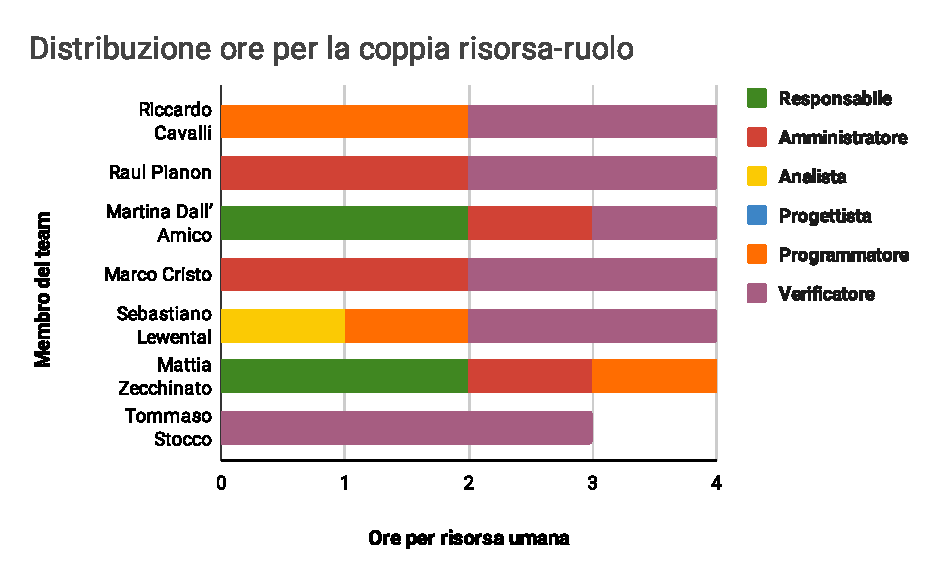
\includegraphics[width=0.90\textwidth]{assets/Consuntivo/Sprint-8/distribuzione_ore_risorsa_ruolo.pdf}
    \caption{Sprint 8 - Istogramma della distribuzione oraria per la coppia risorsa-ruolo}
  \end{figure}

  \begin{figure}[H]
    \centering
    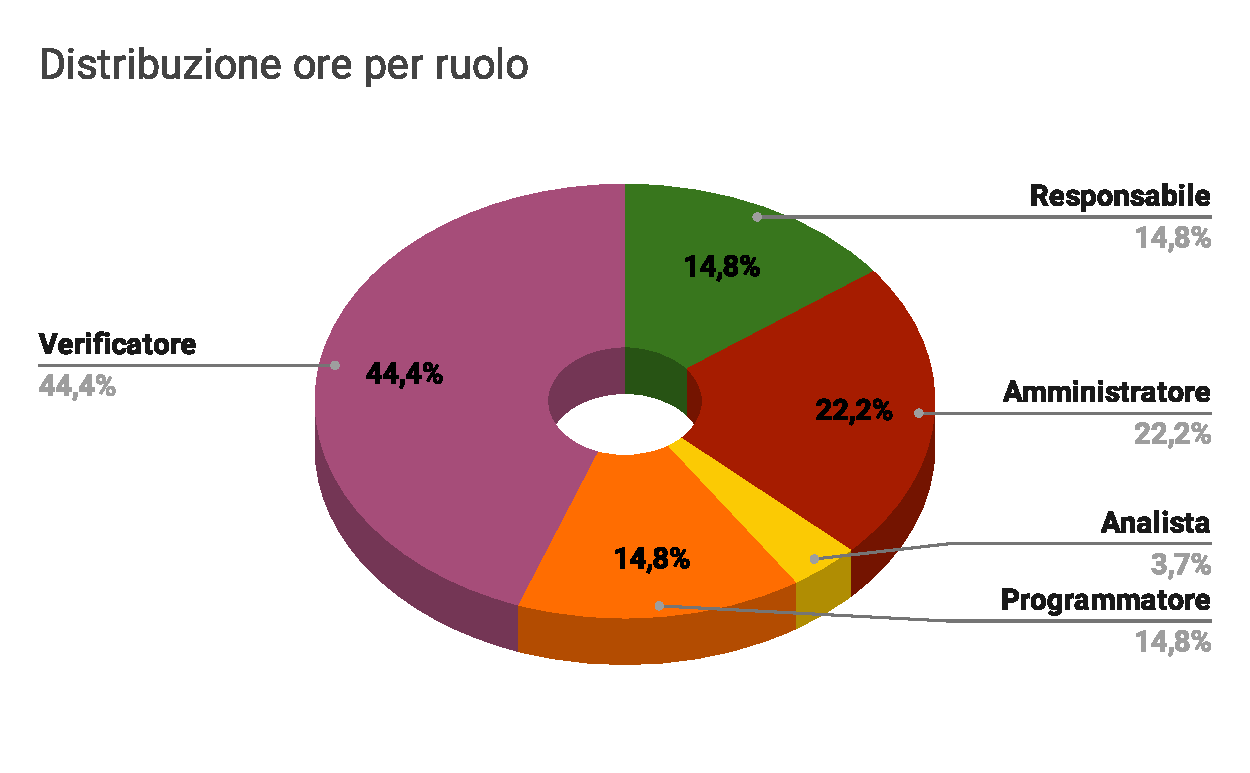
\includegraphics[width=0.90\textwidth]{assets/Consuntivo/Sprint-8/distribuzione_ore_ruolo.pdf}
    \caption{Sprint 8 - Areogramma della distribuzione oraria per ruolo}
  \end{figure}

  \begin{minipage}{\textwidth}
  Di seguito è riportato il consuntivo economico dell'ottavo \glossario{sprint}:
  \begin{table}[H]
  \begin{adjustwidth}{-0.5cm}{-0.5cm}
    \centering
    \begin{tabular}{|P{2.9cm}|P{2.3cm}|P{2.5cm}|P{2.3cm}|>{\arraybackslash}P{2.5cm}|}
      \hline
      \multicolumn{5}{|c|}{\textbf{Consuntivo economico}} \\
      \hline
      \textbf{Ruolo} & \textbf{Ore per ruolo} & \textbf{Delta ore preventivo - consuntivo} & \textbf{Costo (in \texteuro)} & \textbf{Delta costo preventivo - consuntivo (in \texteuro)} \\
      \hline
      Responsabile & 4 & -1 & 120,00 & -30,00 \\ \hline
      Amministratore & 6 & 1 & 120,00 & 20,00 \\ \hline
      Analista & 1 & 1 & 25,00 & 25,00 \\ \hline
      Progettista & 0 & 0 & 0,00 & 0,00 \\ \hline
      Programmatore & 4 & 0 & 60,00 & 0,00 \\ \hline
      Verificatore & 12 & 0 & 180,00 & 0,00 \\ \hline
      \textbf{Totale} & \textbf{27} & 1 & \textbf{505,00} & 15,00 \\ \hline
      \textbf{Restante} & 325 & / & 6.500,00 & / \\ \hline
      \textbf{Sprint pregressi} & 294 & / & 6.015,00 & / \\ \hline
    \end{tabular}
    \caption{Sprint 8 - Consuntivo economico}
  \end{adjustwidth}
  \end{table}
  \end{minipage}

  \begin{figure}[H]
    \centering
    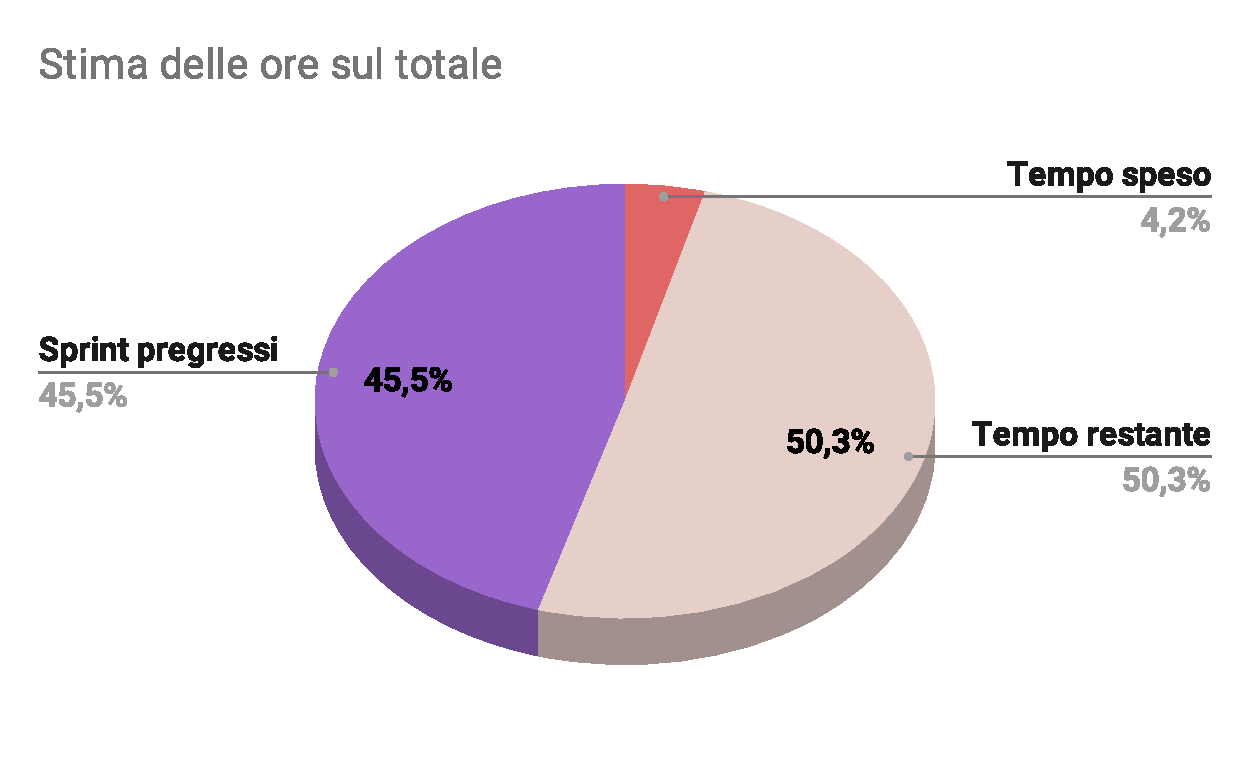
\includegraphics[width=0.90\textwidth]{assets/Consuntivo/Sprint-8/copertura_oraria.pdf}
    \caption{Sprint 8 - Areogramma del tempo speso (in ore) rispetto al totale}
  \end{figure}

  \begin{figure}[H]
    \centering
    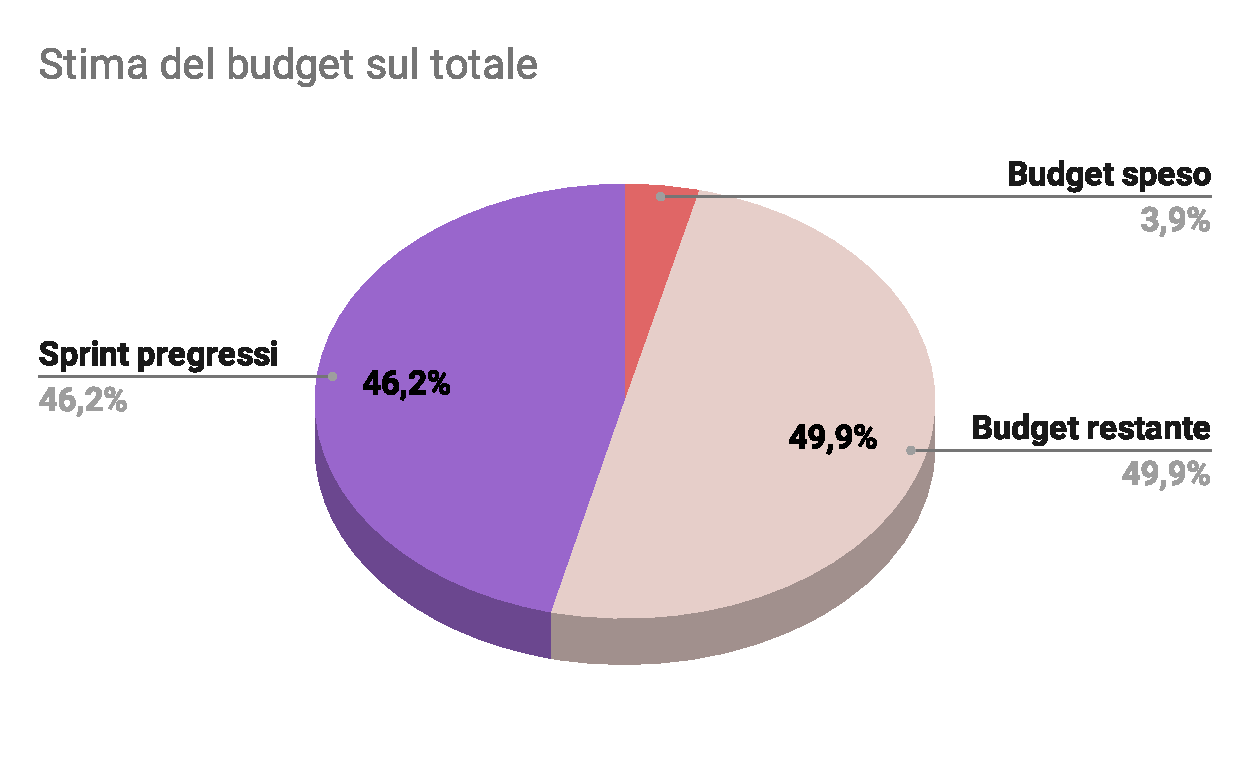
\includegraphics[width=0.90\textwidth]{assets/Consuntivo/Sprint-8/budget_speso.pdf}
    \caption{Sprint 8 - Areogramma del budget speso rispetto al totale}
  \end{figure}

  \begin{minipage}{\textwidth}
    Di seguito sono riportate le ore rimanenti per la coppia risorsa-ruolo:
    \begin{table}[H]
      \begin{tabularx}{\textwidth}{|c|*{6}{>{\centering}X|}c|}
        \hline
        \multicolumn{8}{|c|}{\textbf{Ore rimanenti per la coppia risorsa-ruolo}} \\
        \hline
        \textbf{Membro del team} & \textbf{Re} & \textbf{Am} & \textbf{An} & \textbf{Pt} & \textbf{Pr} & \textbf{Ve} & \textbf{Totale per persona} \\
        \hline
        Cavalli Riccardo & 0 & 0 & 4 & 14 & 11 & 11 & 40 \\
        \hline
        Pianon Raul & 2 & 3 & 1 & 20 & 9 & 9 & 44 \\
        \hline
        Dall’Amico Martina & 3 & 1 & 1 & 14 & 16 & 11 & 46 \\
        \hline
        Cristo Marco & 2 & 6 & 1 & 17 & 10 & 10 & 46 \\
        \hline
        Lewental Sebastiano & 5 & 4 & 1 & 11 & 14 & 12 & 47 \\
        \hline
        Zecchinato Mattia & 5 & 2 & 3 & 11 & 13 & 14 & 48 \\
        \hline
        Stocco Tommaso & 5 & 0 & 3 & 20 & 9 & 15 & 52 \\
        \hline
        \textbf{Totale ore per ruolo} & 22 & 17 & 14 & 107 & 83 & 82 & \textbf{325} \\
        \hline
      \end{tabularx}
      \caption{Sprint 8 - Ore rimanenti per la coppia risorsa-ruolo}
    \end{table}
  \end{minipage}

\subsubsection{Revisione delle attività}

Nell'arco dell'ottavo \glossario{sprint}, il team ha svolto le seguenti attività:
\begin{itemize}
  \item Aggiornamento della documentazione in preparazione alla prima fase della revisione \glossario{RTB};
  \item Completamento \glossario{PoC};
  \item Revisione delle metriche di processo e di prodotto;
  \item Suddivisione delle metriche in base all'obiettivo.
\end{itemize}

\subsubsection{Retrospettiva}

\par Di seguito sono riportati i risultati del questionario di valutazione dello \glossario{sprint}:
\begin{itemize}
  \item Organizzazione dello \glossario{sprint}\ - Valutazione: 8;
  \item Conduzione dei meeting interni - Valutazione: 8;
  \item Conduzione dei meeting esterni - Valutazione: 8;
  \item Impegno e partecipazione dei singoli membri - Valutazione: 3;
  \item La quasi totalità dei membri del team era a conoscenza delle proprie mansioni;
  \item La numerosità delle riunioni è risultata adeguata per tutti i membri del gruppo;
  \item Le riunioni sono state organizzate quasi sempre con il giusto preavviso;
  \item Il rapporto ore spese/ore produttive si sta notevolmente equilibrando;
  \item La produttività è stata ragioneole considerando le criticità della sessione.
\end{itemize}

\vspace{0.5\baselineskip}
\par A seguire le \textbf{analisi a posteriori} dell'ottavo \glossario{sprint}:
\begin{itemize}
  \item TODO.
\end{itemize}

\paragraph*{Pianificazione futura:}
\par Si è deciso di mantenere moderata la quantità di ore assegnate a ciascun membro del team, in modo da continuare a garantire un equilibrio tra lavoro e studio. Confermdo lo stato del progetto si è deciso di fissare gli appuntamenti relativi la \glossario{RTB} nel prossimo sprint.

\paragraph*{Preventivo "a finire" (\sezione{sec:stima_temporale}):}
\par L'avanzamento dello stato prodotto porta a stabilire l'organizzazione della revisione RTB durante il prossimo \glossario{sprint}.

\paragraph*{Gestione dei rischi (\sezione{sec:analisi_rischi}):}
\vspace{0.5\baselineskip}
\par Durante l'ottavo \glossario{sprint}, i seguenti rischi sono stati gestiti con successo:
\begin{itemize}
  \item \textbf{RP1 - Questioni personali}: alcuni membri del gruppo hanno dovuto affrontare questioni personali che hanno impattato sulla loro partecipazione alle attività. Tuttavia, la flessibilità del team ha permesso di riallocare le risorse in modo da garantire il rispetto delle scadenze;
  \item \textbf{RT3 - Malfunzionamenti software}: gli errori sono stati risolti mediante la ricostruzione delle immagini Docker, in conformità con le specifiche definite nel README caricato nel repository ChatSQL.
\end{itemize}
